\documentclass[a4paper]{article}

%%\usepackage{showframe}
\usepackage{graphicx}
\usepackage{float}

\usepackage[ngerman]{babel}

\usepackage[utf8]{inputenc}

\usepackage[useregional]{datetime2}

\usepackage{csquotes}

\usepackage[T1]{fontenc}
%\renewcommand*\familydefault{\sfdefault} %% Only if the base font of the document is to be sans serif

\usepackage{geometry}
\geometry{
 a4paper,
 left=20mm,
 right=20mm,
 bottom=30mm,
 top=30mm
}

\newcommand{\Version}{1.3.1}

\makeatletter
\title{Standard-Setup für NinjaFirewall}\let\Title\@title
\author{Daniel Ruf}\let\Author\@author
\date{26. Februar 2022} \let\Date\@date
\makeatother

\usepackage[a-1b]{pdfx}
\begin{filecontents*}{\jobname.xmpdata}
  \Title{\Title\ v\Version\ (\Date)}
  \Author{\Author}
  \Language{de-DE}
  \Keywords{}
  \Publisher{}
  \Subject{\Title\ v\Version\ (\Date)}
\end{filecontents*}

\usepackage{hyperref}
\hypersetup{
  colorlinks=true,
  linkcolor=blue,
  filecolor=blue,
  urlcolor=blue
}
\urlstyle{same}

\usepackage{fancyhdr}

\pagestyle{fancy}
\fancyhf{}

\begin{document}
\lhead{\Title}
\lfoot{v\Version}
\rfoot{\today}

\noindent

%%{\fontfamily{cmss}\selectfont

\noindent
\textbf{Schritt 1:} installiere und aktiviere NinjaFirewall

\begin{figure}[H]
  \centering
  \includegraphics[width=0.85\textwidth]{images/1.png}
\end{figure}

\noindent
\textbf{Schritt 2:} gehe zu NinjaFirewall -- Event Notifications und kopiere die Kontakt-Emailadresse

\begin{figure}[H]
  \centering
  \includegraphics[width=0.85\textwidth]{images/2.png}
\end{figure}

\noindent
\textbf{Schritt 3:} gehe zu \href{https://danielruf.github.io/ninjafirewall-config-browser/}{ninjafirewall config browser}

\begin{figure}[H]
  \centering
  \includegraphics[width=0.85\textwidth]{images/3.png}
\end{figure}

\newpage

\noindent
\textbf{Schritt 4:} füge die Kontakt-Emailadresse ein und klick den Download-Button

\begin{figure}[H]
  \centering
  \includegraphics[width=0.85\textwidth]{images/4.png}
\end{figure}

\noindent
\textbf{Schritt 5:} gehe zu NinjaFirewall -- Firewall Options

\begin{figure}[H]
  \centering
  \includegraphics[width=0.85\textwidth]{images/5.png}
\end{figure}

\noindent
\textbf{Schritt 6:} importiere die heruntergeladene Konfigurations-Datei

\begin{figure}[H]
  \centering
  \includegraphics[width=0.85\textwidth]{images/6.png}
\end{figure}

\begin{figure}[H]
  \centering
  \includegraphics[width=0.85\textwidth]{images/7.png}
\end{figure}

\noindent
\textbf{Schritt 7:} speicher das Formular (in manchen Fällen müssen Schritt 6 und 7 wiederholt werden)

\begin{figure}[H]
  \centering
  \includegraphics[width=0.85\textwidth]{images/8.png}
\end{figure}

\noindent
\textbf{Schritt 8:} gehe zu NinjaFirewall -- Event Notifications, alle Events sollten angehakt sein

\begin{figure}[H]
  \centering
  \includegraphics[width=0.85\textwidth]{images/9.png}
\end{figure}

\newpage

\noindent
\textbf{Schritt 9:} gehe zu NinjaFirewall -- Dashboard

\begin{figure}[H]
  \centering
  \includegraphics[width=0.85\textwidth]{images/10.png}
\end{figure}

\noindent
\textbf{Schritt 10:} klick auf \enquote{activate Full WAF mode}

\begin{figure}[H]
  \centering
  \includegraphics[width=0.85\textwidth]{images/11.png}
\end{figure}

\noindent
\textbf{Schritt 11:} speicher das Formular (runterscrollen um den Button zu sehen, die ausgewählten Einstellungen sollten ok sein)

\begin{figure}[H]
  \centering
  \includegraphics[width=0.85\textwidth]{images/12.png}
\end{figure}

\noindent
\textbf{Schritt 12:} NinjaFirewall wird eine .user.ini Datei auf der Ebene von wp-config.php erstellen

\begin{figure}[H]
  \centering
  \includegraphics[width=0.85\textwidth]{images/13.png}
\end{figure}

\newpage

\noindent
\textbf{Schritt 13:} nach ein paar Minuten sollte der Status aktualisiert sein (Seite neuladen)

\begin{figure}[H]
  \centering
  \includegraphics[width=0.85\textwidth]{images/14.png}
\end{figure}

\noindent
\textbf{Schritt 14:} gehe zu NinjaFirewall -- Monitoring

\begin{figure}[H]
  \centering
  \includegraphics[width=0.85\textwidth]{images/15.png}
\end{figure}

\noindent
\textbf{Schritt 15:} erstell einen Snapshot

\begin{figure}[H]
  \centering
  \includegraphics[width=0.85\textwidth]{images/16.png}
\end{figure}

\newpage

\noindent
\textbf{Schritt 16:} setz das Scan-Intervall auf täglich

\begin{figure}[H]
  \centering
  \includegraphics[width=0.85\textwidth]{images/17.png}
\end{figure}

\noindent
\textbf{Schritt 17:} klick den Speichern-Button

\begin{figure}[H]
  \centering
  \includegraphics[width=0.85\textwidth]{images/18.png}
\end{figure}

\noindent
\textbf{Schritt 18:} gehe zu File Guard auf der gleichen Seite

\begin{figure}[H]
  \centering
  \includegraphics[width=0.85\textwidth]{images/19.png}
\end{figure}

\noindent
\textbf{Schritt 19:} aktivier File Guard und klick den Speichern-Button

\begin{figure}[H]
  \centering
  \includegraphics[width=0.85\textwidth]{images/20.png}
\end{figure}

\newpage

\noindent
\textbf{Schritt 20:} öffne ein neues Inkognito-Fenster im Browser und öffne deine-domain/wp-content/index.php?f=\%00,
die Anfrage sollte blockiert werden und dort sollte die folgende Information von NinjaFirewall zu sehen sein,
die unten auch die Event-ID enthält
%%\indent bottom.

\begin{figure}[H]
  \centering
  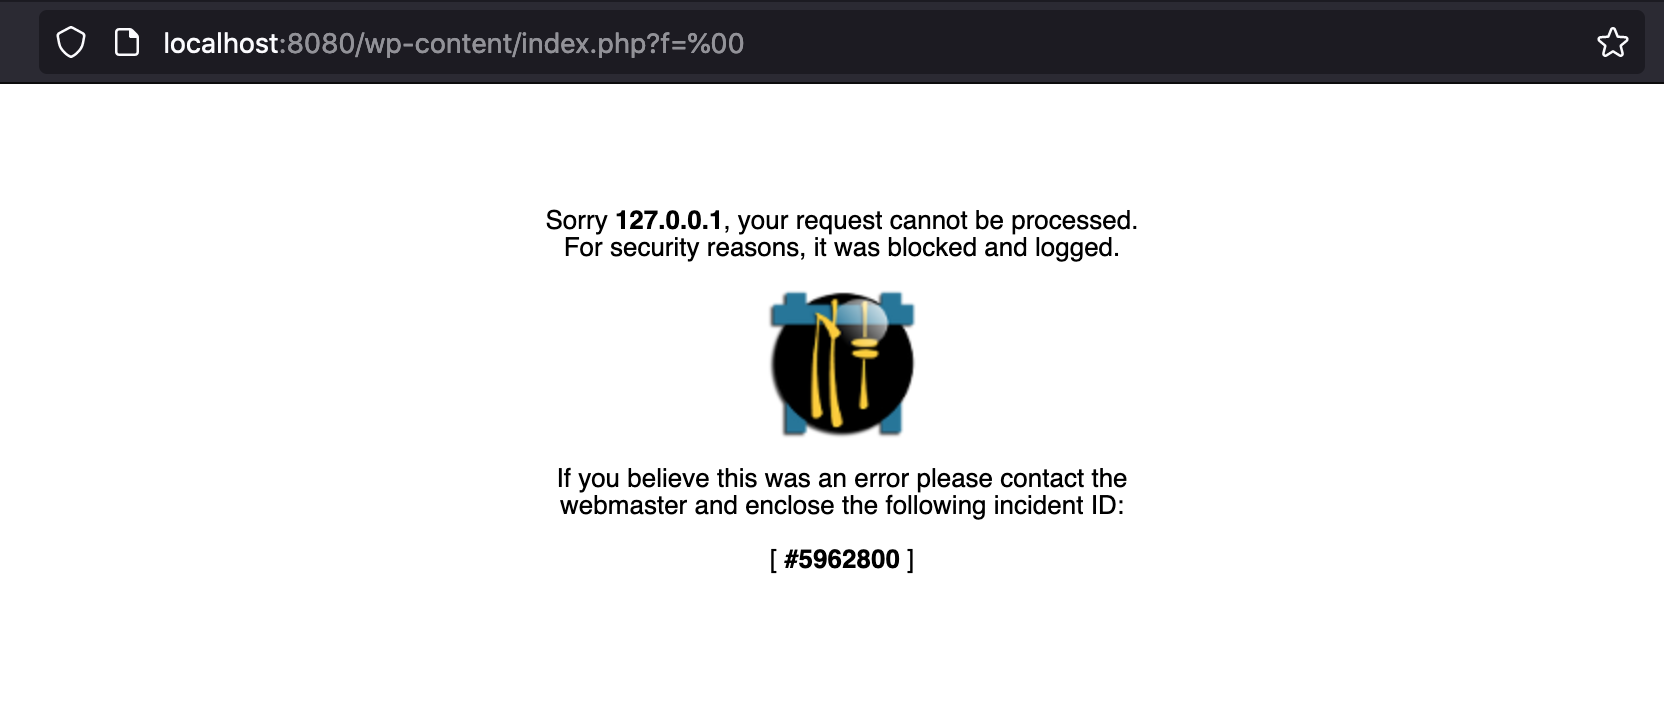
\includegraphics[width=0.85\textwidth]{images/21.png}
\end{figure}

\noindent
\textbf{Schritt 21:} gehe zu NinjaFirewall -- Logs, die blockierte Anfrage sollte jetzt dort auftauchen

\begin{figure}[H]
  \centering
  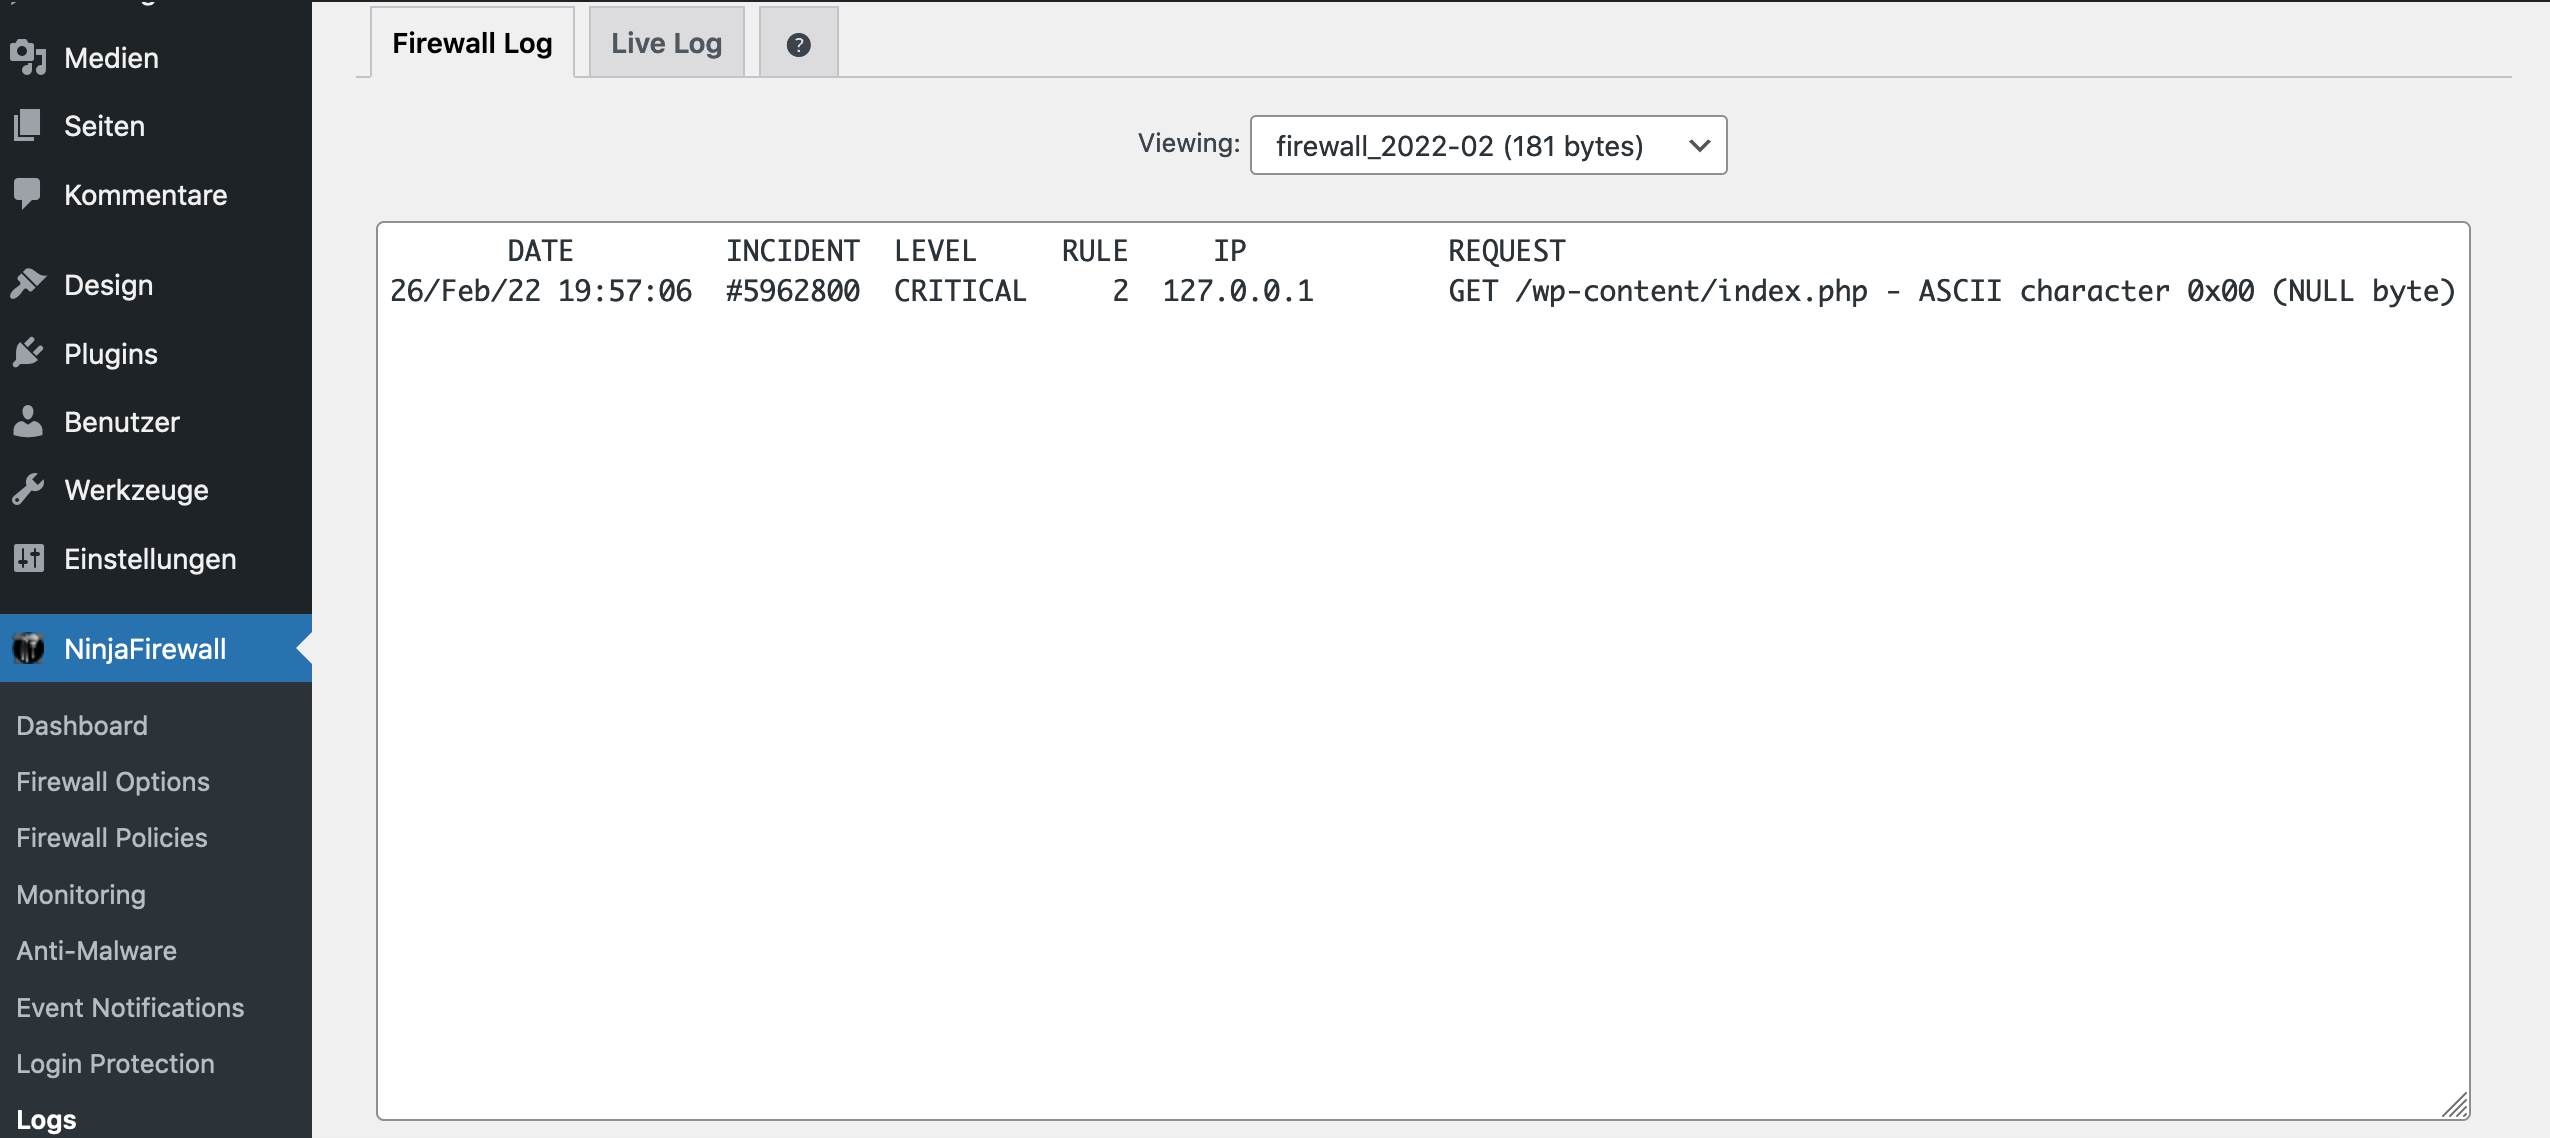
\includegraphics[width=0.85\textwidth]{images/22.png}
\end{figure}

\newpage

\noindent
\textbf{Schritt 22 (optional):} gehe zu NinjaFirewall -- Login Protection und verwende die folgenden Optionen

\begin{figure}[H]
  \centering
  \includegraphics[width=0.85\textwidth]{images/23.png}
\end{figure}

%%}

\end{document}
